\section{Experiments}
\label{sec:exp}
We compare our models with several kinds of baselines on two different datasets. And we analyse the influence of OOV issue, the number of external documents and domain adaptation ability.

\subsection{Two Datasets}

We choose two typical categories, dress and bag, and create two datasets. For each dataset, we use the same method to obtain gold segmented queries and external documents. Using dress dataset as example, we collect brand names, product names, attribute names and attribute values in this category and build a small size dictionary. Then a simple max matching algorithm is used to segment queries in the query log with the help of the dictionary. To ensure the quality of such automatically generated labels, we only reserve queries that can be divided perfectly. In other words, all segments of these chosen queries must appear in the dictionary. External documents are some descriptive documents about some dress products which can crawled from online shopping platforms.

For dress dataset, we collect about 25k queries for training and 1.8k queries for test. The number of documents is 10k. For bag category, about 20k and 2k queries are for training and test respectively. The number of external documents is 15k. Fig \ref{fig:12} shows length distributions of segments and queries using dress dataset as example. Note that the length of a segment is the number of characters in the segment, while the length of a query is the number of segments.


\begin{figure}
	\centering
	\begin{subfigure}[b]{0.45\columnwidth}
		\centering
		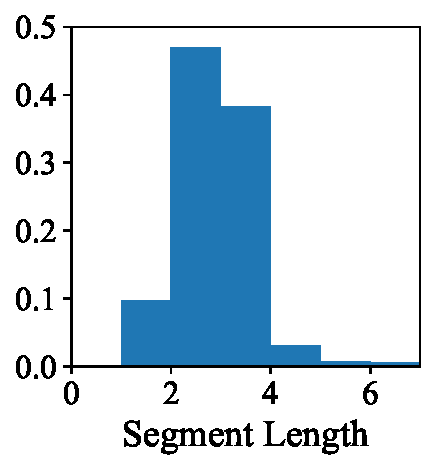
\includegraphics[width=0.8\columnwidth]{figures/data-1.pdf}
		\caption{Distribution of segments.}
		\label{fig:1}
	\end{subfigure}
	\hfill
	\begin{subfigure}[b]{0.45\columnwidth}
		\centering
		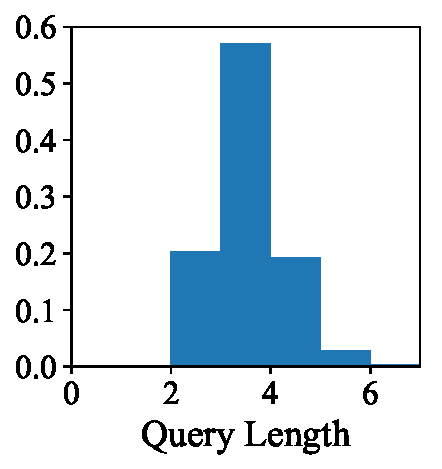
\includegraphics[width=0.8\columnwidth]{figures/data-2.pdf}
		\caption{\small Distribution of queries.}
		\label{fig:2}
	\end{subfigure}
	\caption{Segment and query length distributions of dress dataset.}
	\label{fig:12}
\end{figure}



\subsection{Implementation Details}

We split $10\%$ queries from training set as validation data. All hyper parameters are tuned on validation data. The character embedding size is tuned from $5$ to $50$ by step $5$. The best embedding size is $10$, which seems really small compared with other deep learning models. The reason is that the character set size in our task is also very small. The hidden size of LSTM cell is $10$ too. And the size of distance embedding is set to $5$. We use the Adam algorithm with the learning rate $0.0001$ to do back propagation. The batch size is set to $32$. All parameters are initialized from standard normal distribution. The upper limit size of context bag is $5$. In other words, if there are more than $5$ contexts found for a character, we only use $5$ contexts randomly.

We choose two kinds of metrics to evaluate segmentation performances. First kind of metrics is common P.R.F. (Precision, Recall and F1) to evaluate the ability to recognize correct segments. Second is Query Accuracy which is the percentage of queries segmented correctly.


\subsection{Baselines}

There are three kinds of baselines, existing tools, unsupervised approaches and supervised approaches. CWS task is very similar to query segmentation, which means the tools trained for CWS can also be applied to query segmentation task directly. We choose three popular and open source CWS tools, SnowNLP\footnote{https://github.com/isnowfy/snownlp}, THULAC \cite{sun2016thulac} and Jieba\footnote{https://github.com/fxsjy/jieba}. As for unsupervised approaches, we implement the model from \cite{risvik_query_2003} called UNS which is based on fequency count and mutual information. UNS is learnt on queries and external documents. UNS(-Queries) and UNS(-Documents) are learnt without queries or external documents respectively. As for supervised approaches, we choose three existing models, Word2Vec-LR \cite{kale_towards_2017} which is a simple deep learning model based on word embedding, traditional feature-based Perceptron model \cite{du_perceptron-based_2014} and CRF model \cite{yu_query_2009}. BiLSTM-CRF(Q) which only relies on hidden vector of characters in a query is also one of our baselines.

\subsection{Results}
\label{sec:results}

% Main table
\begin{table*}[h!]
	\centering
	\small
	\caption{Evaluation metrics of all baselines and our models on two datasets.}
	\begin{tabular}{lcccccccc}% {c|ccc|c | ccc|c}
		\toprule
		\multirow{2}{*}{Models} & \multicolumn{4}{c}{Dress} & \multicolumn{4}{c}{Bag}                                                                                                       \\
		\cmidrule(lr){2-5} \cmidrule(lr){6-9}
		                        & Precision                 & Recall                  & F1             & Query Accuracy & Precision      & Recall         & F1             & Query Accuracy \\
		\midrule
		SnowNLP                 & 0.287                     & 0.448                   & 0.350          & 0.074          & 0.242          & 0.403          & 0.303          & 0.116          \\
		THULAC                  & 0.459                     & 0.572                   & 0.509          & 0.291          & 0.385          & 0.488          & 0.431          & 0.333          \\
		Jieba                   & 0.478                     & 0.614                   & 0.538          & 0.275          & 0.469          & 0.586          & 0.521          & 0.387          \\
		\midrule
		UNS                     & 0.427                     & 0.428                   & 0.427          & 0.221          & 0.377          & 0.404          & 0.390          & 0.294          \\
		UNS(-Queries)           & 0.542                     & 0.469                   & 0.503          & 0.326          & 0.350          & 0.385          & 0.366          & 0.268          \\
		UNS(-Documents)         & 0.292                     & 0.234                   & 0.260          & 0.117          & 0.206          & 0.180          & 0.192          & 0.132          \\
		\midrule
		Word2Vec-LR             & 0.687                     & 0.597                   & 0.639          & 0.470          & 0.661          & 0.685          & 0.672          & 0.587          \\
		Perceptron              & 0.650                     & 0.639                   & 0.644          & 0.499          & 0.826          & 0.831          & 0.828          & 0.798          \\
		CRF                     & 0.659                     & 0.642                   & 0.650          & 0.503          & 0.847          & 0.840          & 0.844          & 0.821          \\
		% \midrule
		BiLSTM-CRF(Q)           & 0.815                     & 0.792                   & 0.804          & 0.705          & 0.802          & 0.805          & 0.803          & 0.760          \\
		\midrule
		BiLSTM-CRF(C)           & 0.834                     & 0.830                   & 0.832          & 0.732          & 0.706          & 0.774          & 0.739          & 0.661          \\
		BiLSTM-CRF(Q+C)         & \textbf{0.855}            & \textbf{0.851}          & \textbf{0.853} & \textbf{0.759} & \textbf{0.868} & \textbf{0.867} & \textbf{0.867} & \textbf{0.837} \\
		\bottomrule
	\end{tabular}
	\label{tab:main}
\end{table*}

As shown in Table \ref{tab:main}, our BiLSTM-CRF(Q+C) is the best model on both dress and bag datasets. In dress category, the best baseline is BiLSTM-CRF(Q), and our BiLSTM-CRF(Q+C) achieves 0.049 improvements in F1 value. In bag category, the best baseline is CRF, and our BiLSTM-CRF(Q+C) beats it by 0.023 in F1 value.

Existing tools trained on open domain sentences for CWS task work really bad for query segmentation in e-commerce field. The data distributions of sentences in CWS and queries in query segmentation are really different. A strange thing is that Jieba is better than THULAC in F1 value but worse in Qeury Accuracy. The reason is that although Jieba can recognize more correct segments, these correct segments are distributed in different queries dispersively. Unsupervised models also work not well, even worse than the existing Jieba tool. Supervised models trained on labelled queries are much better than other baselines. BiLSTM-CRF(Q) and feature-based CRF are two best baselines. BiLSTM-CRF(Q) beats CRF by 0.154 on dress dataset in F1 value, while CRF beats BiLSTM-CRF(Q) by 0.041 on bag dataset.

The effectiveness of our added contexts from external documents can be proved from two aspects. BiLSTM-CRF(C) which predicts labels only on the information from contexts can still work not bad. BiLSTM-CRF(C) even is better than the best baseline on dress dataset. This means the boundary information in contexts can be used to segment queries independently. From another perspective, BiLSTM-CRF(Q) can work much better after adding contexts. By comparing BiLSTM-CRF(Q+C) with BiLSTM-CRF(Q), contexts bring  0.049 and 0.064 improvements in F1 value on dress and bag datasets respectively.

To get more details on the training process, Fig \ref{fig:curve} shows the growth of F1 value of BiLSTM-CRF(Q), BiLSTM-CRF(C) and BiLSTM-CRF(Q+C). Due to early stop strategy, the stop epoch of different models are different.

\begin{figure}[th]
	\centering
	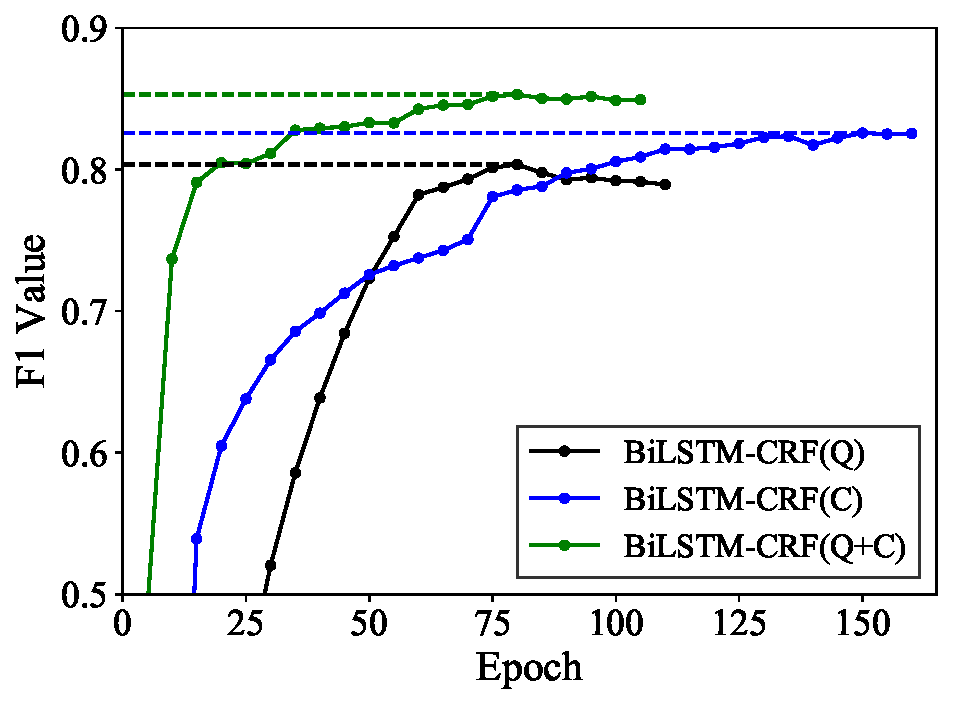
\includegraphics[width=0.7\columnwidth]{figures/result-1.pdf}
	\caption{The learning trends of BiLSTM-CRF(Q), BiLSTM-CRF(C) and BiLSTM-CRF(Q+C).}
	\label{fig:curve}
\end{figure}


\subsection{Discussions}

\subsubsection{Out-Of-Vocabulary}
\label{sec:oov}

Out-of-Vocabulary (OOV) is a common challenge of many NLP tasks. OOV rate is the proportion of out-of-vocabulary segments. The OOV rates of dress and bag datasets are $85.3\%$ and $29.4\%$ respectively, which means the OOV issue of dress dataset is much more severe than bag dataset. Most of segments in test queries are not seen in training queries for dress dataset, while most of segments in test queries appear in training queries for bag dataset. To measure the influence of OOV issue, we split all segments in test queries into two kinds, IV (in-vocabulary) segments and OV (out-vocabulary) segments. Similar to normal recall metric, we calculate the recall of IV segments (Recall-IV) and recall of OV segments (Recall-OV) independently. Recall-IV is the percentage of correctly predicted IV segments, while Recall-OV is the percentage of correct OV segments.

As shown in Table \ref{tab:oov}, for every model, Recall-IV is much higher than Recall-OV which means segments appearing in training queries are much easier to be recognized. This proves that OOV issue also has huge impact on query segmentation task. As for Recall-IV, our BiLSTM-CRF(Q+C) works near the same as the best baseline model. On dress dataset, BiLSTM-CRF(Q+C) beats the best baseline by a small margin 0.008, while on bag dataset, BiLSTM-CRF(Q+C) loss to the best baseline also by a small margin 0.002. However, as for Recall-OV, our BiLSTM-CRF(Q+C) is much better than all baselines by a large margin. This large gain is due to the extra boundary information contained in contexts. These OV segments can not be found in training queries which mean almost no features about OV segments can be extracted just from training queries. With the help of external documents, some features of OV segments may be extracted from contexts.

In section \ref{sec:results}, we have mentioned BiLSTM-CRF(Q) is the best baseline on dress dataset in F1 value while CRF is the best baseline on bag dataset. The main reason is that OOV rate of bag dataset is much lower than dress dataset. When the OOV rate is low, CRF model can work much better on IV segments than BiLSTM-CRF(Q). This cause CRF model beats BiLSTM-CRF(Q) in F1 value on bag dataset.

% Both BiLSTM-CRF and DiSQuS($z_i=[h_i;b_i]$) can achieve a really good recall for IV words. But DiSQuS($z_i=[h_i;b_i]$) defeats BiLSTM-CRF in Recall-OV value with a large margin, which make DiSQuS($z_i=[h_i;b_i]$) better than BiLSTM-CRF in final F1 value. The reason is that DiSQuS approach can still extract enough features for OV words from the document corpus, while other baseline models can only rely on OV words themselves.

% Vocabulary
\begin{table}[th]
	\centering
	\small
	\caption{\small The Recall-IV and Recall-OV of unsupervised, supervised and our models on two dataset.}
	\begin{tabular}{lcccc}
		\toprule
		\multirow{2}{*}{Models} & \multicolumn{2}{c}{Dress} & \multicolumn{2}{c}{Bag}                                   \\
		\cmidrule(lr){2-3} \cmidrule(lr){4-5}
		                        & IV                        & OV                      & IV             & OV             \\
		\midrule
		UNS                     & 0.642                     & 0.407                   & 0.354          & 0.427          \\
		UNS(-Queries)           & 0.661                     & 0.451                   & 0.331          & 0.409          \\
		UNS(-Documents)         & 0.315                     & 0.226                   & 0.155          & 0.192          \\

		\midrule
		Word2Vec-LR             & 0.768                     & 0.581                   & 0.814          & 0.626          \\
		Perceptron              & 0.887                     & 0.595                   & 0.891          & 0.685          \\
		CRF                     & 0.882                     & 0.600                   & \textbf{0.892} & 0.714          \\
		% \midrule
		BiLSTM-CRF(Q)           & 0.938                     & 0.778                   & 0.859          & 0.780          \\
		\midrule
		BiLSTM-CRF(C)           & 0.901                     & 0.823                   & 0.765          & 0.778          \\
		BiLSTM-CRF(Q+C)         & \textbf{0.946}            & \textbf{0.842}          & 0.890          & \textbf{0.856} \\
		\bottomrule
	\end{tabular}
	\label{tab:oov}
\end{table}


\subsubsection{The Number of External Documents}

The core strength of our models is that they can take advantage of contexts from external documents. The number of external documents will decide the probability that a character in a query can find contexts. The more documents we have, the more likely a character can find contexts. We use the proportion of characters which have at least 1 contexts to evaluate the average probability of finding contexts in the documents.

In order to eliminate the interference of hidden state of characters in queries, we choose BiLSTM-CRF(C) without $h_i$ to study the effect of the number of documents. As shown in Fig \ref{fig:alpha}, with the growth of the number of external documents, the probability increases, which means more contexts can be found. Then the performance of BiLSTM-CRF(C) also increases.

\begin{figure}[th]
	\centering
	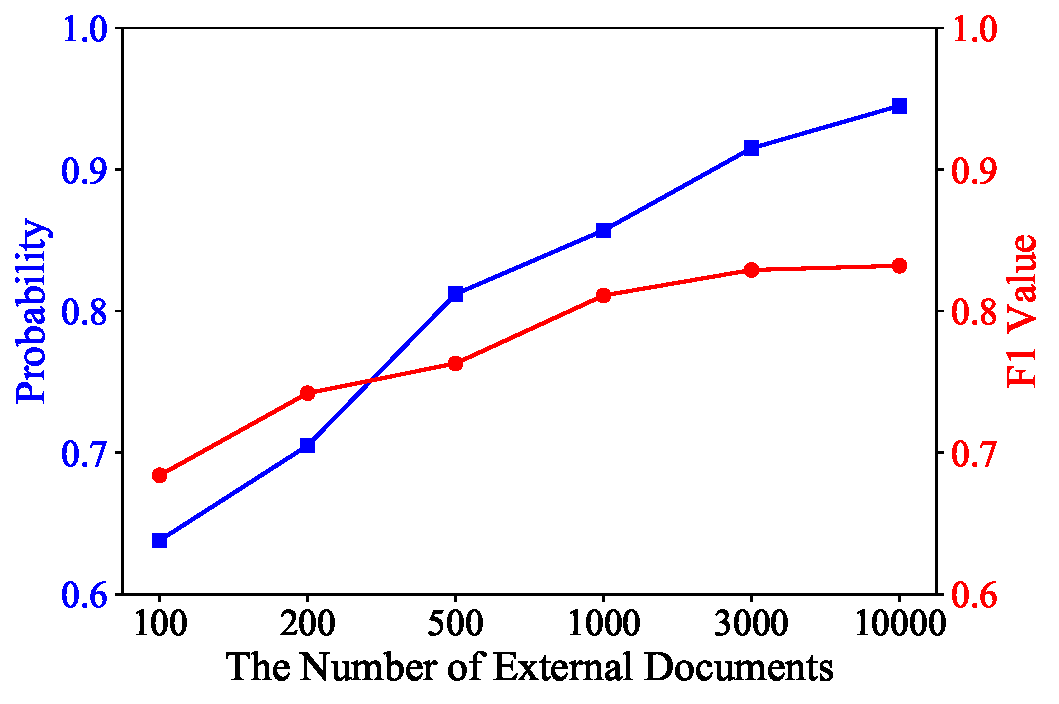
\includegraphics[width=0.7\columnwidth]{figures/result-2.pdf}
	\caption{With the increase of the number of external documents, the bule line shows the change of probability that at least 1 contexts can be found, and the red line shows the change of F1 value of BiLSTM-CRF(C).}
	\label{fig:alpha}
\end{figure}


\subsubsection{Domain Adaptation}

Most of supervised models perform well on the dataset where they are trained and tuned on, but suffer a huge performance drop in another domain. We argue that adding the contexts from external documents can bring a better domain adaptation ability to basic BiLSTM-CRF(Q). We compare BiLSTM-CRF(Q+C) with BiLSTM-CRF(Q) by training the model on one dataset and testing on another dataset.

In Table \ref{tab:domain}, $dataset_1 \rightarrow dataset_2$ means the model is trained on $dataset_1$ and tested on $dataset_2$. We only show the F1 value of each model. Diff indicates the difference between $dataset_1 \rightarrow dataset_1$ and $dataset_1 \rightarrow dataset_2$, which represents the performance drop due to domain adaptation from $dataset_1$ to $dataset_2$. When the training set is dress and test set is bag, BiLSTM-CRF(Q+C) achieves lower decline than BiLSTM-CRF(Q). This advantage can be more obvious when training set is bag and test set is dress.
% Domain adaptation
\begin{table}[th]
	\centering
	\small
	\caption{D and B are the abbreviations of dress and bag datasets respectively. The values in the table are F1 value.}
	\begin{tabular}{lcccc}
		\toprule
		Models          & D $\rightarrow$ D & D $\rightarrow$ B & Diff  \\
		\midrule
		BiLSTM-CRF(Q)   & 0.804             & 0.531             & 0.273 \\
		BiLSTM-CRF(Q+C) & 0.853             & 0.634             & 0.219 \\
		\bottomrule
		\toprule
		Models          & B $\rightarrow$ B & B $\rightarrow$ D & Diff  \\
		\midrule
		BiLSTM-CRF(Q)   & 0.803             & 0.428             & 0.375 \\
		BiLSTM-CRF(Q+C) & 0.867             & 0.752             & 0.115 \\
		\bottomrule
	\end{tabular}
	\label{tab:domain}
\end{table}



